\documentclass{article}
\usepackage[utf8]{inputenc}
\usepackage{indentfirst}
\usepackage{titling}
\usepackage{geometry}
\usepackage{graphicx}
\graphicspath{ {./Images/} }
\usepackage[shortlabels]{enumitem}
\usepackage{fancyhdr}
\usepackage{ulem}
\usepackage[dvipsnames]{xcolor}
\usepackage{amssymb}
\usepackage{listings}
\usepackage{color}

\definecolor{dkgreen}{rgb}{0,0.6,0}
\definecolor{gray}{rgb}{0.5,0.5,0.5}
\definecolor{mauve}{rgb}{0.58,0,0.82}

\lstset{frame=tb,
  language=Java,
  aboveskip=3mm,
  belowskip=3mm,
  showstringspaces=false,
  columns=flexible,
  basicstyle={\small\ttfamily},
  numbers=none,
  numberstyle=\tiny\color{gray},
  keywordstyle=\color{blue},
  commentstyle=\color{dkgreen},
  stringstyle=\color{mauve},
  breaklines=true,
  breakatwhitespace=true,
  tabsize=3
}

\def\ojoin{\setbox0=\hbox{$\bowtie$}%
  \rule[-.02ex]{.25em}{.4pt}\llap{\rule[\ht0]{.25em}{.4pt}}}
\def\leftouterjoin{\mathbin{\ojoin\mkern-5.8mu\bowtie}}
\def\rightouterjoin{\mathbin{\bowtie\mkern-5.8mu\ojoin}}
\def\fullouterjoin{\mathbin{\ojoin\mkern-5.8mu\bowtie\mkern-5.8mu\ojoin}}

\renewcommand\maketitlehooka{\null\mbox{}\vfill} %para centralizar verticalmente
\renewcommand\maketitlehookd{\vfill\null}
\pagestyle{fancy}
\fancyhf{}
\rfoot{\thepage}
\lfoot{ 
\includegraphics[scale=0.01]{UA.jpg} José Mendes 107188 LEI}
\geometry{
  a4paper,
  headheight=4cm,
  top=5.5cm,
  bottom=4.5cm,
  footskip=4cm
}


\title{Introdução à Engenharia de Software}
\author{José Mendes 107188}
\date{2023/2024}

\begin{document}


\begin{titlepage}
    \maketitle
    \begin{center}
        
\includegraphics[scale=0.4]{UA.png}
    \end{center}
    \thispagestyle{empty} %remove o count da pagina
\end{titlepage}

\pagebreak

\section{Maven}

\subsection{O que é o Maven?}

É uma \textbf{ferramenta de gestão de projetos}, que inclui:
\begin{itemize}
  \item Um \textbf{project object model} (POM) que descreve o projeto;
  \item Um conjunto de \textbf{standards};
  \item Um \textbf{lifecycle} do projeto;
  \item Um sistema de gestão de \textbf{dependências};
  \item Lógica para \textbf{executar plugins} em \textbf{fases} específicas
  do ciclo de vida.
\end{itemize}

Convenção sobre configuração (layout do projeto é padronizado).

\subsection{Layout de Diretórios Padronizado}

\begin{flushleft}
  \textbf{POM} - Contém uma descrição completa do projeto de como
  construir o projeto.

  \vspace{2mm}

  \textbf{src} - Diretório que contém todo o código fonte para construir
  o projeto, o seu site, \dots

  \vspace{2mm}

  \textbf{target} - Diretório que contém os resultados da construção,
  tipicamente um JAR ou WAR, juntamente com os ficheiros intermedios.
\end{flushleft}

\subsection{POM}

Maven é baseado no conceito de um \textbf{Project Object Model} (POM).
Este é um ficheiro XML, que está sempre localizado no diretório base do projeto
como \textbf{pom.xml} (os users definiram POMs que estendem o Super POM).

O POM contém informação sobre o projeto e vários detalhes de configuração
usados pelo Maven para construir o projeto.

O POM é declarativo, não necessita de detalhes de procedimento.

\subsubsection{Estrutura do POM}

\begin{flushleft}
  O POM contém 4 categorias de descrição e configuração:
  
  \begin{itemize}
    \item Informação geral do projeto, isto é, informação human-readable;
    \item Configuração do build, que pode incluir, adicionar plugins,
    afixar plugins objetivo ao ciclo de vida;
    \item Ambiente de construção, que descreve o ambiente "familiar" em que o Maven está;
    \item Relações POM, isto é, coordenadas, herança, agregação, dependências.
  \end{itemize}
\end{flushleft}

\pagebreak

\subsection{Coordenadas Maven}

As coordenadas definem o lugar único do projeto no universo Maven.
São compostas por 3 partes: \textbf{$<$groupId$>$}, \textbf{$<$artifactId$>$} e
\textbf{$<$version$>$} (The Maven trinity!).

\vspace{2mm}

As versões de um projeto são usadas para agrupar e ordenar lançamentos:

\[ <major\_version>.<minor\_version>.<incremental\_version>-<qualifier> \]

\begin{flushleft}
  \textbf{Exemplo:} 1.0.0-SNAPSHOT ou 1.2.3-alpha-2
\end{flushleft}

Se o qualifier contiver a palavra chave SNAPSHOT, então o Maven
vai expandir este token para uma data e hora convertida para o formato UTC.

\vspace{2mm}

\begin{flushleft}
  \begin{itemize}
    \item \textbf{groupId} - Nome da empresa, organização, equipa, \dots,
    normalmente usando a convenção de nomes de domínio invertidos (reverse URL naming, ex: org.apache.maven);

    \item \textbf{artifactId} - Nome único do projeto dentro do groupId;
    
    \item \textbf{version} - Versão do projeto;
    \item \textbf{packaging} - Tipo de empacotamento do projeto (jar (default), war, \dots);
    \item \textbf{classifier} - Classificador opcional para distinguir artefactos
  \end{itemize}

  \vspace{2mm}

  \textbf{Nota:} As coordenadas Maven identificam unicamente um projeto.
\end{flushleft}

\subsection{Ciclo de Vida Maven}

Um ciclo de vida é uma sequência organizada de fases,
que dão ordem a uma sequência de objetivos.
Estes objetivos são empacotados em plugins que estão ligados
as fases.

\begin{center}
  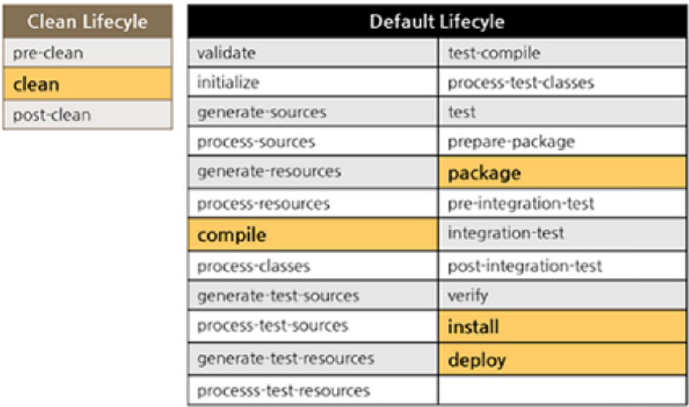
\includegraphics[scale=0.5]{1}
\end{center}

Chamar uma fase específica num ciclo de construção, vai executar
todas as fases anteriores a essa fase.

\pagebreak

\begin{center}
  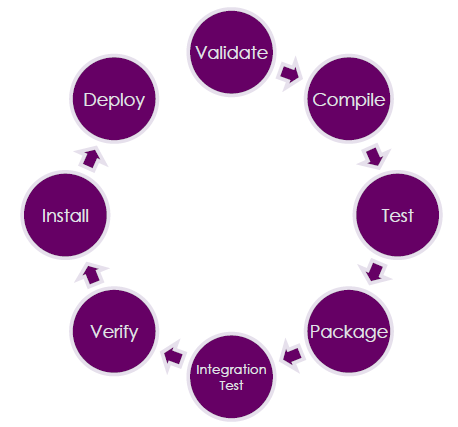
\includegraphics[scale=0.5]{2}
\end{center}

\begin{flushleft}
  \begin{enumerate}
    \item \textbf{Validate} - Valida que a estrutura do projeto está correta.
    (ex: verifica se todas as dependências foram transferidas e estão disponíveis
    no repositório local);

    \item \textbf{Compile} - Compila o código fonte, converte os ficheiros
    \textbf{.java} em \textbf{.class}, e armazenando-os no diretório \textbf{target/classes};

    \item \textbf{Test} - Corre testes unitários para o projeto;
    \item \textbf{Package} - Empacota o código compilado num formato distribuível
    como \textbf{JAR} ou \textbf{WAR};

    \item \textbf{Integration Test} - Corre testes de integração para o projeto;
    \item \textbf{Verify} - Corre verificações para verificar que o projeto é válido
    e que cumpre os critérios de qualidade;

    \item \textbf{Install} - Instala o código empacotado
    no repositório Maven local, para uso como dependência noutros projetos locais;

    \item \textbf{Deploy} - Copia o pacote final de código para o repositório
    remoto para partilha com outros developers e projetos.
  \end{enumerate}
\end{flushleft}

\subsection{Ciclo de Vida de Construção}

O processo para contruir e distribuir um projeto. Consiste
em vários passos designados por \textbf{fases}.

Algumas fases default são:
\begin{itemize}
  \item \textbf{validate}
  \item \textbf{compile}
  \item \textbf{test}
  \item \textbf{package}
  \item \textbf{deploy}
\end{itemize}

\pagebreak

\subsection{Goals e Plugins}

Os Goals são operações fornecidas pelas ferramentas Maven.

Cada fase é uma sequência de Goals, em que cada Goal é responsável
por uma tarefa específica. Quando corremos uma fase, todos os Goals
ligados a essa fase são executados, na ordem em que estão definidos.

\begin{flushleft}
  Algumas Maven Plugins:
  \begin{itemize}
    \item resources
    \item compiler
    \item surefire
    \item jar, war
  \end{itemize}
\end{flushleft}

\subsection{Arquétipos (Archetypes)}

Um Archetype é um template para um projeto Maven, que pode ser usado para
criar um novo projeto rapidamente.

\begin{flushleft}
  \textbf{Exemplo:} \textit{maven-archetype-quickstart} ou \textit{maven-archetype-webapp}
\end{flushleft}

Users podem criar os seus próprios Archetypes e publicá-los através de catálogos.

\subsection{Gestor de Dependências}

Uma \textbf{dependência} de um projeto é uma biblioteca da qual
o projeto depende. Adicionar uma dependência ao projeto é simples,
basta adicionar a dependência ao POM. O Maven vai automaticamente
procurar a dependência no repositório local, e se não encontrar,
vai procurar no repositório remoto e transferi-la.

\begin{center}
  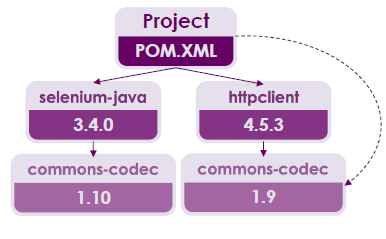
\includegraphics[scale=0.6]{3}
\end{center}

\pagebreak

\section{Git e GitHub}

\subsection{Sistemas de Controlo de Versões}

Um sistema de controlo de versões (também conhecido como sistema de controlo de código fonte) faz o seguinte:
\begin{itemize}
  \item Mantém várias (antigas e novas) versões de tudo (não só código fonte);
  \item Pede por comentários quando se fazem alterações;
  \item Permite "check-in" e "check-out" de ficheiros para saber
  em que ficheiros outras pessoas estão a trabalhar;
  \item Mostra as diferenças entre versões;
\end{itemize}

\subsubsection{Vantagens}

\begin{flushleft}
  \textbf{Ao trabalhar sozinho:} Fornece uma "máquina do tempo" para
  voltar atrás para uma versão anterior, e fornece um bom suporte 
  de diferentes versões do mesmo projeto.

  \vspace{2mm}

  \textbf{Ao trabalhar em equipa:} Simplifica muito trabalhar em concurrencia,
  dando "merge" de alterações feitas por diferentes pessoas.
\end{flushleft}

\subsection{o que é Git e GitHub}

\begin{center}
  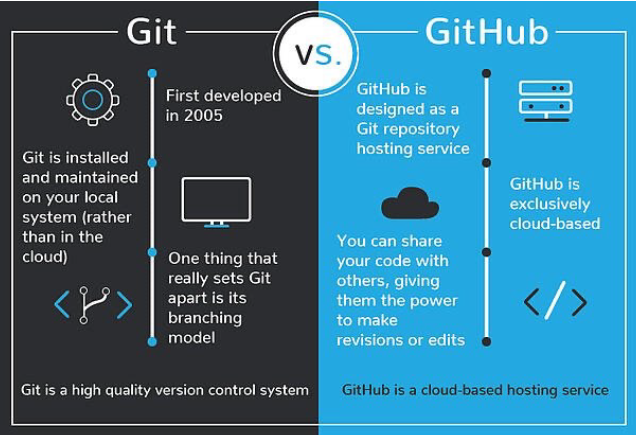
\includegraphics[scale=0.5]{4}
\end{center}

Quando fazemos "git init" num diretório de um projeto, ou quando fazemos
"git clone" de um projeto existente, o Git cria um repositório (.git).

Em qualquer momento, podemos fazer um "snapshot" de tudo
no dirétorio do projeto e guardar este no repositório.
Este "snapshot" é chamado de \textbf{commit object}.

\pagebreak

Um \textbf{commit} ocorre quando fazemos alterações que estão
prontas para serem guardadas no repositório.

Quando realizamos um commit, o Git guarda um \textbf{commit object}:
\begin{itemize}
  \item Um estado completo do projeto, incluindo todos os ficheiros;
  \item O primeio não possui pai;
  \item Normalmente, pegamos num commit object, fazemos alterações,
  e criamos um novo commit object, pelo que a maior parte dos commit objects
  têm apenas um pai;
  \item Quando fazemos \textbf{merge} de dois commit objects,
  forma um commit object com dois pais.
\end{itemize}

Pelo que, os commit objects formam uma \textbf{DAG} (Directed Acyclic Graph).
O Git é tudo sobre usar e manipular este grafo.

\subsubsection{Mensagem de Commit}

Os commits são "baratos" pelo que os devemos fazer com frequência, e com
mensagens descritivas sobre o que foi alterado. Devem ter apenas uma linha.

Como não devemos dizer muito numa linha, devemos fazer vários commits.

\begin{center}
  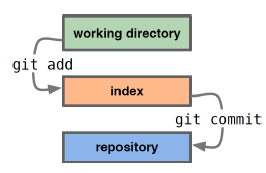
\includegraphics[scale=0.6]{5}
\end{center}

\subsection{Manter simples}

\begin{center}
  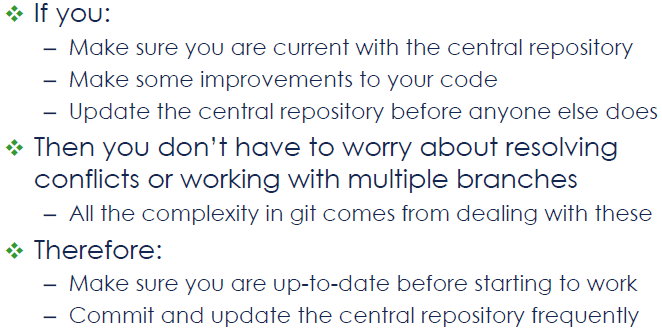
\includegraphics[scale=0.6]{6}
  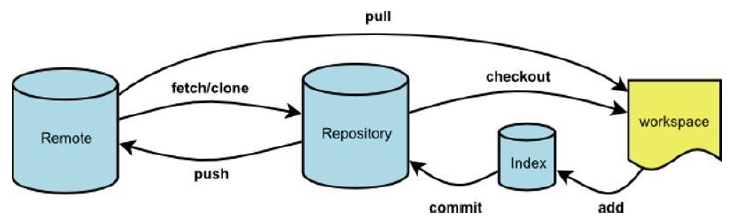
\includegraphics[scale=0.6]{7}
\end{center}

\pagebreak

\section{O Processo de Desenvolvimento de Software}

\subsection{Processo}

A fundação para a Engenharia de Software é a camada de processo.
Um processo de Software é uma framework para as atividades,
ações, e tarefas necessárias para construir software de alta qualidade.
Define as técnicas e a framework de gestão para aplicação de métodos,
ferramentas e pessoas ao longo do processo de desenvolvimento.

\begin{center}
  
\includegraphics[scale=0.6]{8}
\end{center}

\subsection{Porquê o Processo de Software?}

\begin{center}
  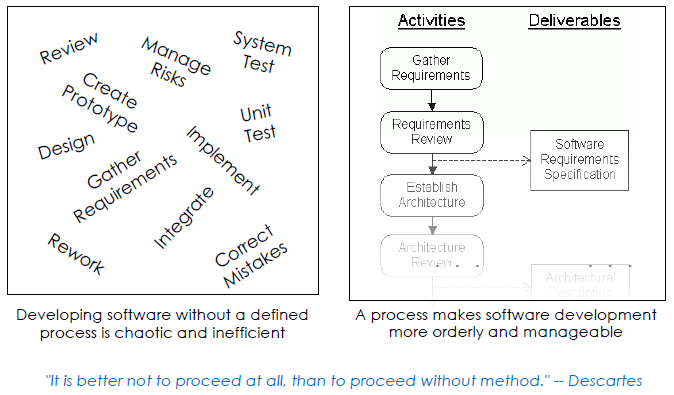
\includegraphics[scale=0.6]{9}
\end{center}

\subsection{Processo de Software}

Existem vários tipos de processos de software, no entanto, todos têm:

\begin{itemize}
  \item \textbf{Especificação (comunicação e planeamento)} - definir o que o sistema deve fazer;
  \item \textbf{Design e Implementação} - definir a organização do sistema e implementar o sistema;
  \item \textbf{Validação} - verificar que faz aquilo que o cliente quer;
  \item \textbf{Evolução} - alterar o sistema em resposta a novos requisitos impostos pelo cliente.
\end{itemize}


Quando discutimos sobre o processo de software, estamos a falar sobre:
\begin{itemize}
  \item \textbf{Atividades} - como especificar um modelo de dados, design de uma
  interface de utilizador, \dots;
  \item \textbf{Ordem} a ordem destas atividades;
\end{itemize}

A descrição de processos pode também incluir, \textbf{produtos} (outcome da
atividade do processo), \textbf{papéis} (roles, responsabilidades das pessoas envolvidas)
e \textbf{pré-/pós-condições} (são condições que são verdadeiras antes
e depois de atividade do processo ou de um produto ser produzido).

\pagebreak

O processo de software específica:
\begin{itemize}
  \item \textbf{O quê}
  \item \textbf{Quem}
  \item \textbf{Quando}
  \item \textbf{Como}
\end{itemize}

E incluí
\begin{itemize}
  \item \textbf{Papéis} (Roles)
  \item \textbf{Fluxo de trabalho} (Workflow)
  \item \textbf{Procedimentos} (Procedures)
  \item \textbf{Normas} (Standards)
  \item \textbf{Modelos} (Templates)
\end{itemize}

\subsection{Pontos Chave}

\textbf{\uline{O processo de Software é um guia}}

\vspace{2mm}

Não existe "um melhor processo para escrever software".
Um processo que um individuo ou uma organização escolhe e segue depende de:
\begin{itemize}
  \item das características específicas do projeto;
  \item da cultura da organização;
  \item das habilidades e preferências das pessoas envolvidas.
\end{itemize}

\vspace{2mm}

Um bom processo aumenta a produtividade de membros da equipa
menos experientes sem impedir o trabalho/progresso de membros
mais experientes.

\subsection{Resistência ao Processo de Software}

\begin{flushleft}
  \textbf{Perceção:} Algumas pessoas vêm seguir um processo como
  uma sobrecarga (overhead) desnecessária na produtividade.
  \begin{itemize}
    \item Interfere com a criatividade;
    \item Burocracia e regimento;
    \item Prejudica a agilidade em mercados que evoluem rapidamente.
  \end{itemize}

  \vspace{2mm}

  \textbf{A realidade:} Grupos que não seguem um processo definido
  tendem a adicionar processo mais tarde no projeto, como reação
  a problemas que surgem. Quando o tamanho e a complexidade do projeto
  aumenta, a importância de seguir processos definidos aumenta proporcionalmente. 
\end{flushleft}

\pagebreak

\subsection{Fases de Software}

\begin{center}
  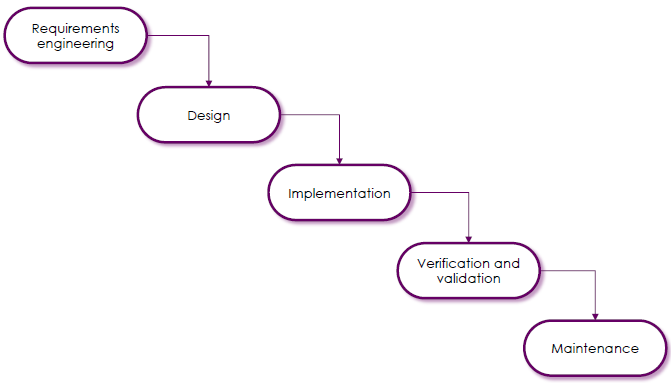
\includegraphics[scale=0.6]{10}
\end{center}

\subsection{\uline{Modelos} de Processo de Software}

Modelos abstratos que descrevem uma classe abordagens de desenvolvimento
com características similares.

\vspace{2mm}

Alguns critérios utilizados para distinguir modelos de processos
de software são:
\begin{itemize}
  \item o tempo entre fases (timing);
  \item critérios de entrada e saída entre fases (entry/exit criteria);
  \item os artefactos criados durante cada fase;
\end{itemize}

\vspace{2mm}

Alguns \textbf{exemplos} incluem: Waterfall, Spiral, Rapid Prototyping,
Incremental, Development, \dots

\subsubsection{Modelos (Tradicionais)}

\begin{flushleft}
  \textbf{Modelo em Cascata (Waterfall):} É um modelo \uline{Plan-Driven}.
  Separa e distingue fases de especificação e desenvolvimento.

  \vspace{2mm}

  \textbf{Desenvolvimento Incremental:} A especificação, desenvolvimento
  e validação são intercalados. Pode ser \uline{Plan-Driven} ou \uline{Agile}.

  \vspace{2mm}

  \textbf{Processos Evolucionários/Iterativos:} O sistema é desenvolvido
  no ínicio usando uma especificação muito simples, sendo modificada
  e melhorada de acordo com as necessidades de software.

  \vspace{2mm}

  \textbf{Muitos outros:} A maior parte de sistemas grandes são desenvolvidos
  usando um processo que incorpora elementos de diferentes modelos.
\end{flushleft}

\pagebreak

\subsubsection{O Modelo em Cascata (Waterfall)}

\begin{center}
  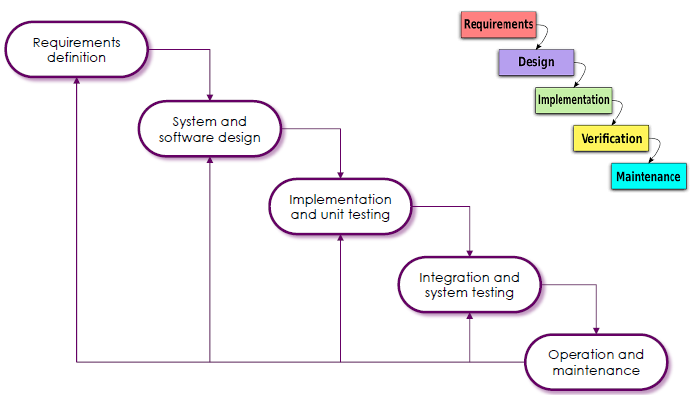
\includegraphics[scale=0.6]{11}
\end{center}

\subsubsection*{Vantagens}

\begin{itemize}
  \item É simples e fácil de perceber e usar;
  \item É fácil de planear, um schedule pode ser definido
  com deadlines para cada fase de desenvolvido e um produto pode ser
  processado através do processo de desenvolvimento como um carro
  numa lavagem automática, e ,teoricamente, ser entregue a tempo.
  \item Fácil de gerir, cada fase tem entregas específicas e um
  processo de revisão.
  \item Fases e processos são concluídos um de cada vez.
  \item Funciona bem onde os requisitos são bem compreendidos.
\end{itemize}

\subsubsection*{Desvantagens}

\begin{itemize}
  \item Dificuldade em acomodar mudanças após o processo começar.
  Em principio, uma fase deve ser concluída antes de começar a próxima.
  Particionamento inflexível do projeto em fases distintas torna difícil
  responder a mudanças nos requisitos do cliente.
  \item Modelo não muito bom para projetos de longa duração ou que já estão em andamento
  (não é produzido nenhum software funcional até mais tarde no ciclo de vida).
  \item Não é adequado a processos onde os requisitos são incertos ou
  onde há risco de serem alterados.
\end{itemize}

\pagebreak

\subsubsection{Modelo Incremental}

Uma característica de modelos com ciclos de vida modernos.
O produto evolui através de uma série de iterações.

\begin{center}
  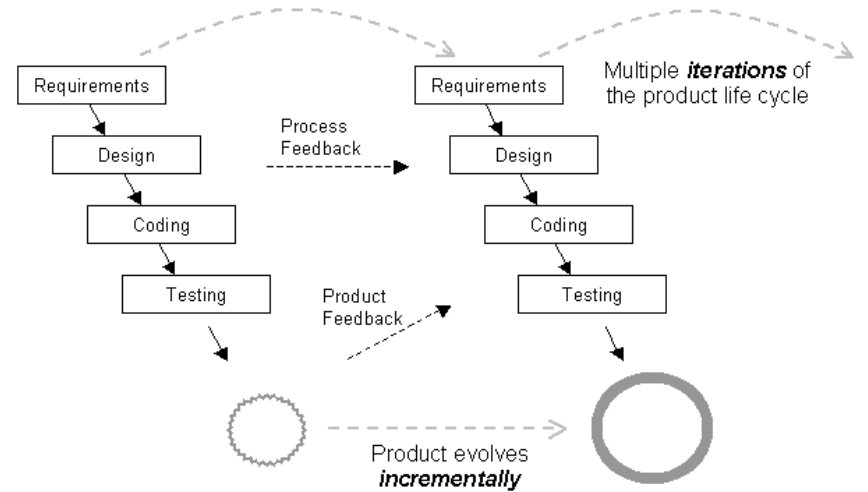
\includegraphics[scale=0.5]{12}
\end{center}

\subsubsection*{Benefícios}

\begin{itemize}
  \item O custo de \textbf{acomodar mudanças de requisitos do cliente} é reduzido.
  A quantidade de análise e documentação que tem de ser refeita é muito menor
  do que no modelo em cascata.

  \item É mais fácil \textbf{obter feedback do cliente} sobre o desenvolvimento
  do trabalho que já está concluído.
  Clientes podem comentar sobre demonstrações do software e ver
  quanto foi implementado.

  \item \textbf{Entrega mais rápida e deployment} do software útil
  para o cliente é possível. Os clientes podem usar e ganhar valor
  do software mais cedo do que se o sistema fosse desenvolvido
  com o processo em cascata.
\end{itemize}

\subsubsection*{Problemas}

\begin{itemize}
  \item \textbf{Cada fase de iteração é rigida} e não se sobrepoem
  umas com as outras.

  \item O processo não é visível. Os gestores precisam  de entragas regulares
  para medir o progresso. No entanto, se o sistema não for desenvolvido rapidamente,
  não é cost-effective produzir documentos que reflitam cada versão do sistema.

  \item A estrutura do sistema tende a degradar-se à medida que novos
  incrementos são adicionados. A não ser que tempo e dinheiro seja
  gasto na refatoração para melhorar o software,
  \textbf{regular mudanças tende a corromper a sua estrutura}.
  A medida que vamos incorporando novas mudanças de doftware,
  torna-se mais difícil e mais caro.
\end{itemize}

\pagebreak

\subsubsection{Modelos Evolucionários/Iterativos}

\begin{flushleft}
  \textbf{Prototipagem:} Geralmente, um cliente define um conjunto
  de objetivos gerais para o software, mas não identifica requisitos
  detalhados para funções e funcionalidades do sistema.

  \vspace{2mm}

  \textbf{Modelo Espiral:} Utilizando um modelo espiral, o software é desenvolvido
  numa serie de lançamentos (releases) evolutivos. Durante as primeiras iterações,
  o lançamento pode ser um protótipo ou um modelo.

  \vspace{2mm}

  \textbf{Modelo Concurrente:} Permite a uma equipa de software representar
  elementos iterativos e concurrentes de quaisquer modelos de processo.
\end{flushleft}

\subsubsection{Incremental vs Evolucionário/Iterativo}

\begin{center}
  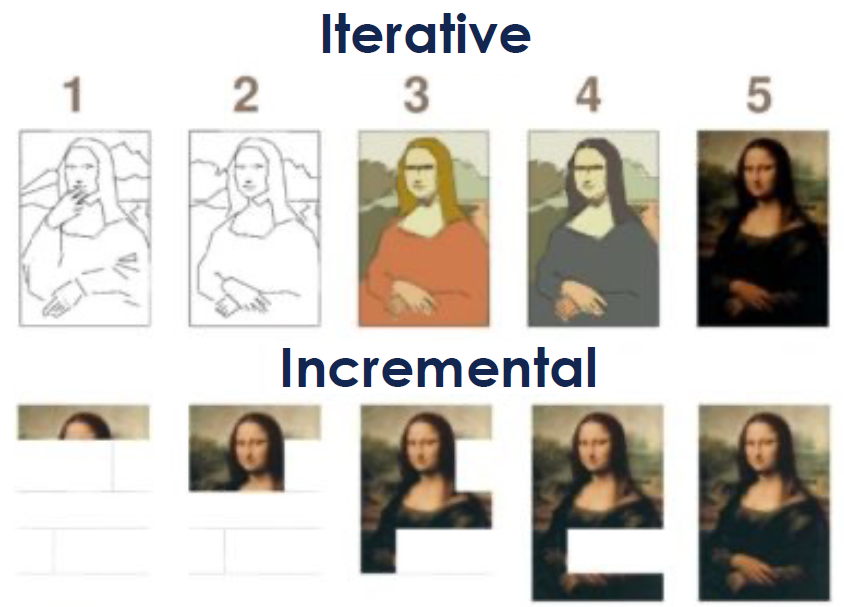
\includegraphics[scale=0.5]{13}
\end{center}

\subsubsection{Exemplos}

\begin{center}
  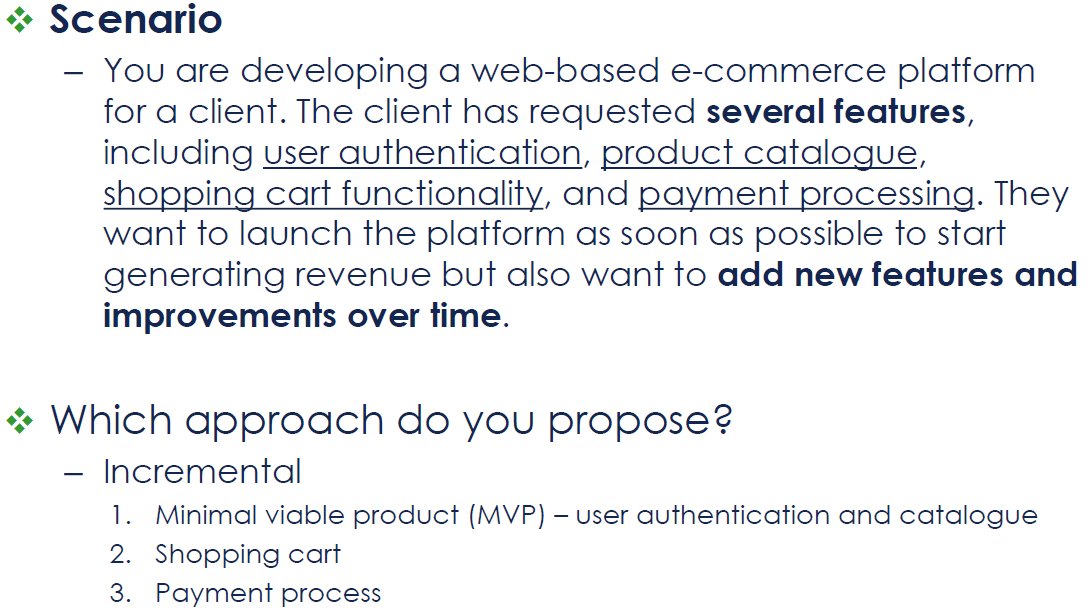
\includegraphics[scale=0.32]{14}
  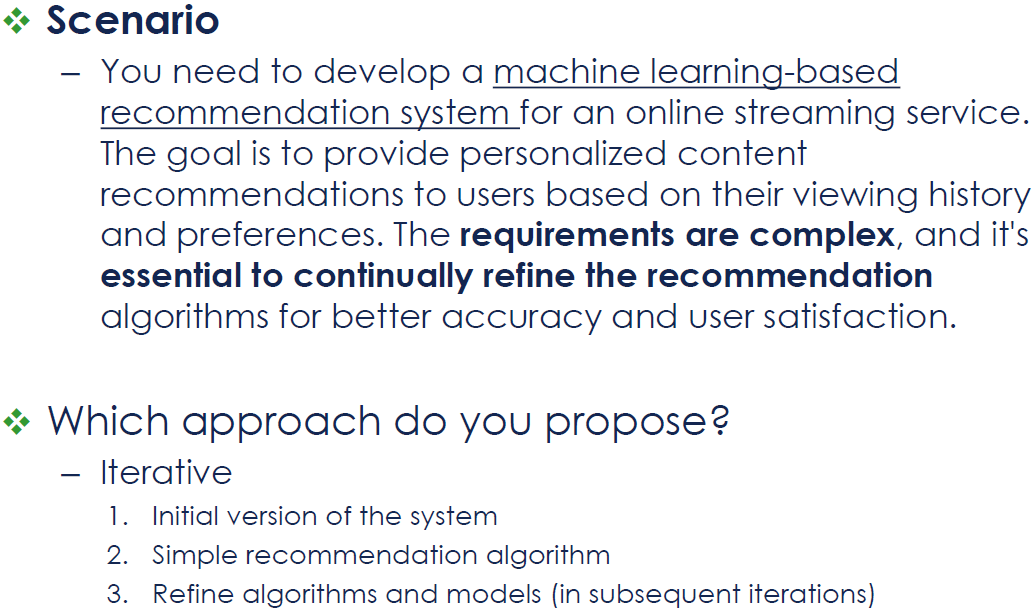
\includegraphics[scale=0.32]{15}
\end{center}

\pagebreak

\subsection{Outros Modelos de Processo}

\begin{itemize}
  \item Desenvolvimento \textbf{Component-Based} (COTS): O processo
  para aplicar quando reutilizar é um objetivo do desenvolvimento.

  \item \textbf{Métodos Formais}: Enfatiza a especificação matemática
  dos requisitos.

  \item \textbf{Processo Unificado (UP)}: Um processo de software
  "use-case driven, arquitetura-centric, iterativo e incremental",
  alinhado com o Unified Modeling Language (UML).
\end{itemize}

\subsection{Processo Unificado (UP)}

\begin{center}
  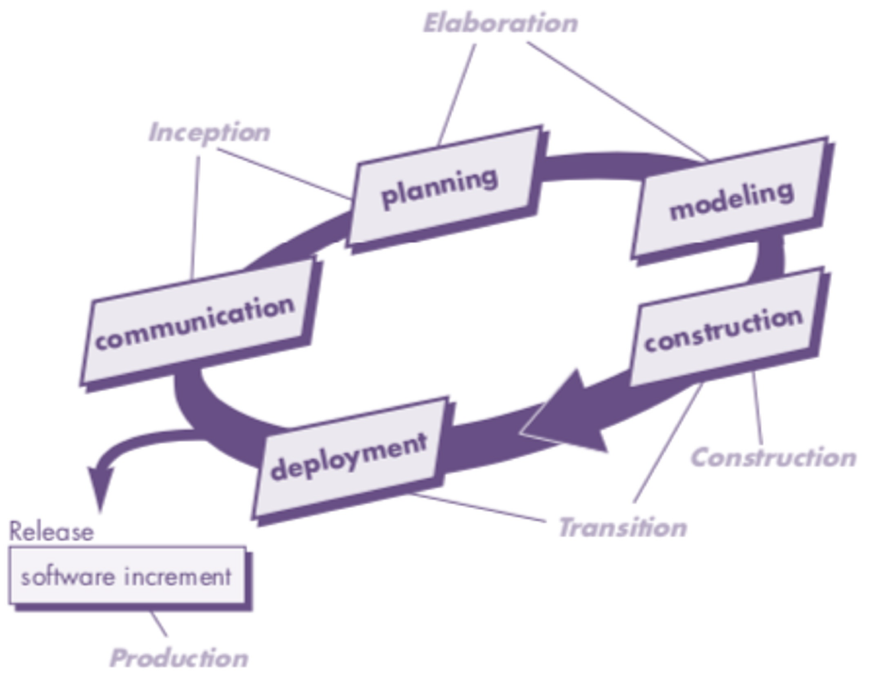
\includegraphics[scale=0.4]{16}
\end{center}

\subsubsection{Fases}

\begin{center}
  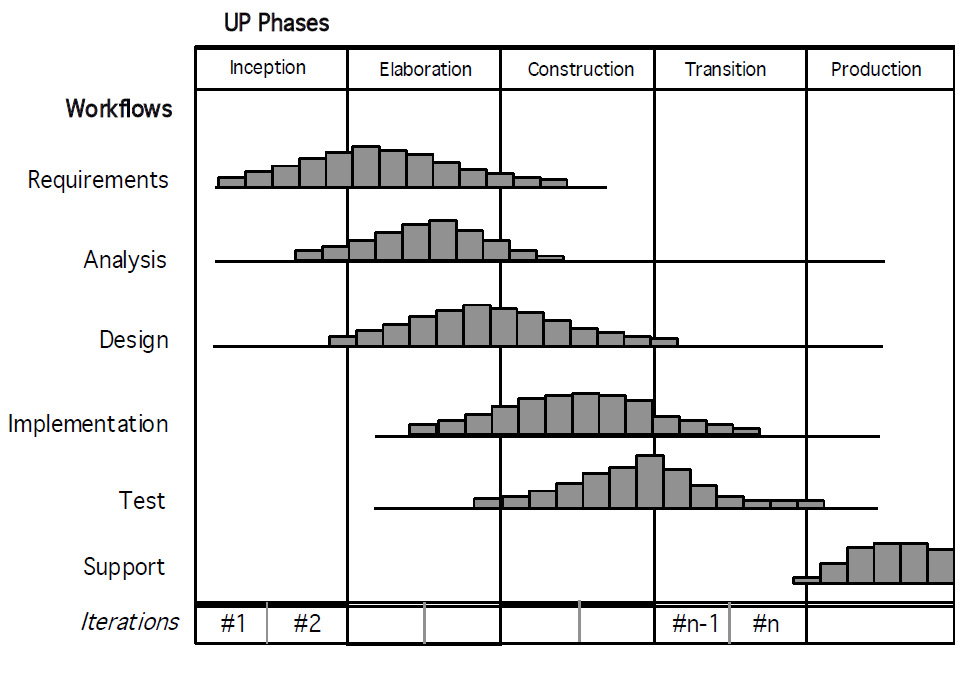
\includegraphics[scale=0.4]{17}
\end{center}

\pagebreak

\subsection{Processos Plan-Driven e Agile}

\textbf{Processos Plan-Driven} são processos onde todas as atividades
são planeadas \uline{anteciadamente} e o progresso é medido
contra este plano.

\vspace{2mm}

Em \textbf{Processos Agile}, planear é incremental e é mais fácil
mudar o processo para refletir a mudança nos requisitos do cliente.

\vspace{2mm}

Na prática, a maior parte dos processos incluem elementos de ambos,
processos plan-driven e agile. Não existem processos de software
"certos" ou "errados".

\subsubsection{Processos Plan-Driven vs Agile}

\begin{center}
  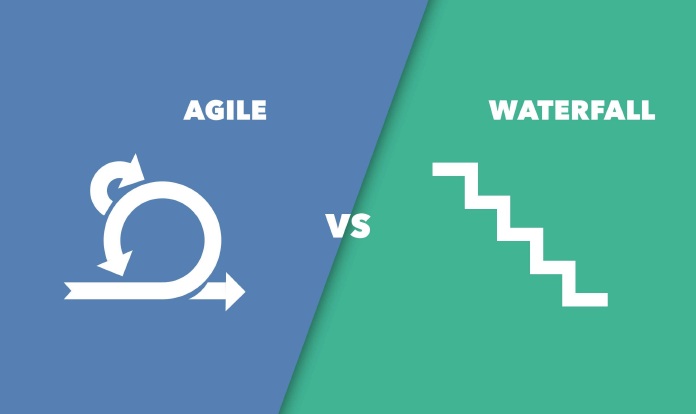
\includegraphics[scale=0.5]{18}
\end{center}

\subsubsection{Processos Agile}

Desenvolvimento rápido e entragas são, geralmente, os requisitos
mais importantes para sistemas de software.
\begin{itemize}
  \item Negócios operam num ambiente \textbf{fast-changing requirements}
  e é praticamente impossível produzir um conjunto de requisitos de software
  estáveis.
  \item O Software deve evoluir rapidamente para refletir mudanças de
  negócios.
\end{itemize}

\vspace{2mm}

Desenvolvimento Plan-Driven é essencialmente para alguns tipos de sistemas
mas não cobre as necessidades do negócio.

\subsubsection*{Métodos Agile}

\begin{itemize}
  \item Métodos Agile foram desenvolvidos num esforço para ultrapassar
  fraquezas percetidas e reais em engenharia de software convencional.
  
  \item \textbf{Foca no código em vez de no design}.
  
  \item Baseados em \textbf{abordagens iterativas} ao desenvolvimento
  de software.

  \item Tem a intenção de \textbf{entregar software funcional rapidamente}
  e evoluir rapidamente para refletir mudanças de requisitos do cliente.
\end{itemize}

\pagebreak

\subsubsection{Origem: Manifesto Agile}

"We are uncovering better ways of developing
software by doing it and helping others do it.
Through this work we have come to value:

\begin{itemize}
  \item \textbf{Individuals and interactions} over processes and tools
  \item \textbf{Working software} over comprehensive documentation
  \item \textbf{Customer collaboration} over contract negotiation
  \item \textbf{Responding to change} over following a plan
\end{itemize}

That is, while there is value in the items on the right,
we value the items on the left more."

\subsubsection{Princípios dos Métodos Agile}

\begin{flushleft}
  \textbf{Involvimento do cliente:} Os clientes devem estar envolvidos
  durante todo o porcesso de desenvolvimento. O seu papel é fornecer
  e priorizar novos requisitos e avaliar as iterações do sistema.
\end{flushleft}

\subsubsection{Desenvolvimento Plan-Driven e Agile}

\begin{center}
  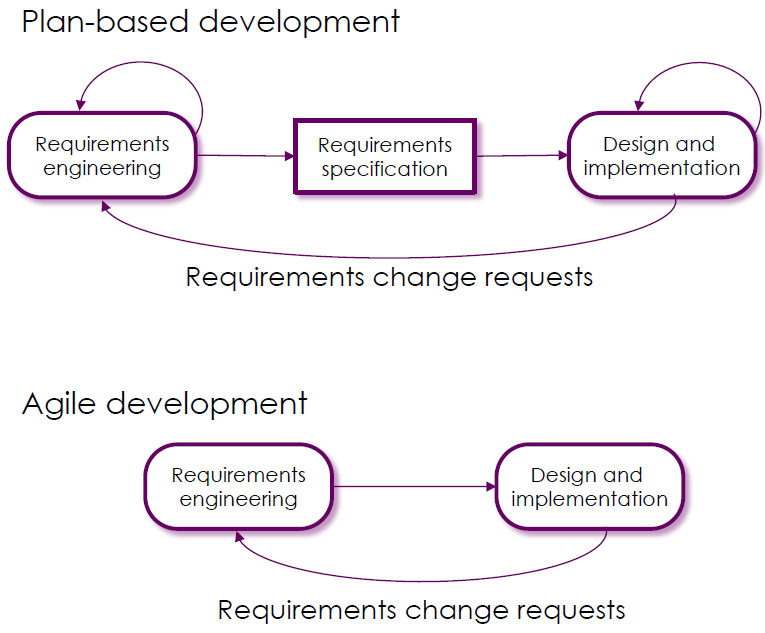
\includegraphics[scale=0.4]{19}
\end{center}

\begin{flushleft}
  \textbf{Desenvolvimento Plan-Driven:}
  \begin{itemize}
    \item Baseado ao redor de um desenvolvimento separado de fases,
    com outputs a serem produzidos em cada fase planeada anteciadamente.
    \item Não é necessariamente o modelo em cascata - desenvolvimento
    incremental, plan-driven, é possível.
  \end{itemize}

  \vspace{2mm}

  \textbf{Desenvolvimento Agile:}
  \begin{itemize}
    \item Especificação, design, implementação e testes são intercalados.
    \item Os outputs do processo de desenvolvimento são decididos
    através de um processo de negociação durante o processo de desenvolvimento
    de software.
  \end{itemize}
\end{flushleft}

\pagebreak

\subsubsection{Métodos Agile - Benefícios}

\begin{itemize}
  \item Requisitos num modelo Agile podem ser alterados
  conforme os requisitos do cliente mudam. Por vezes os requisitos
  não são muito claros. Mudanças nos requisitos são aceites
  mesmo em fases avançadas do processo de desenvolvimento.

  \item A entrega de software é continua. Clientes podem seguir
  cada feature funcional do Sprint do software.

  \item Refatorar o código não é muito caro.
\end{itemize}

\subsubsection{Métodos Agile - Desvantagens}

\begin{itemize}
  \item A documentação é escassa.
  \item Com requisitos pouco claros, é difícil estimar o resultado pretendido.
  Mais díficil de estimar o esforço necessário.
  \item Alguns riscos desconhecidos/imprevisiveis que podem afetar o desenvolvimento do projeto. 
\end{itemize}

\subsubsection{Métodos Agile - Aplicabilidade}

\begin{itemize}
  \item Desenvolvimento de produtos, onde uma empresa de software está a desenvolver
  um produto pequeno/médio em tamanho para venda.

  \item Desenvolvimento de sistemas customizados dentro de uma organização,
  onde existe o compromisso do cliente ficar envolvido no processo de desenvolvimento
  e onde existem algumas regras/regulamentos externos que afetam o software.
  
  \item Virtualmente, todos os produtos de software e aplicações são desenvolvidas
  usando abordagens Agile.
\end{itemize}

\pagebreak

\section{Desenvolvimento de Software Agile}

\subsection{Princípios Agile}

\subsubsection{Porquê Agile?}

O desenvolvimento rápido e entrega são, geralmente, os requisitos
mais importantes para sistemas de software.
\begin{itemize}
  \item Negócios operam num ambiente \textbf{fast-changing requirements}
  e é praticamente impossível produzir um conjunto de requisitos de software
  estáveis.
  \item O Software deve evoluir rapidamente para refletir mudanças de
  negócios.
\end{itemize}

\vspace{2mm}

Princípios Agile:
\begin{itemize}
  \item \textbf{Focada no código em vez de no design};
  \item Baseados em \textbf{abordagens iterativas} ao desenvolvimento
  de software;
  \item Tem a intenção de \textbf{entregar software funcional rapidamente}
  e evoluir rapidamente para refletir mudanças de requisitos do cliente.
\end{itemize}

\begin{center}
  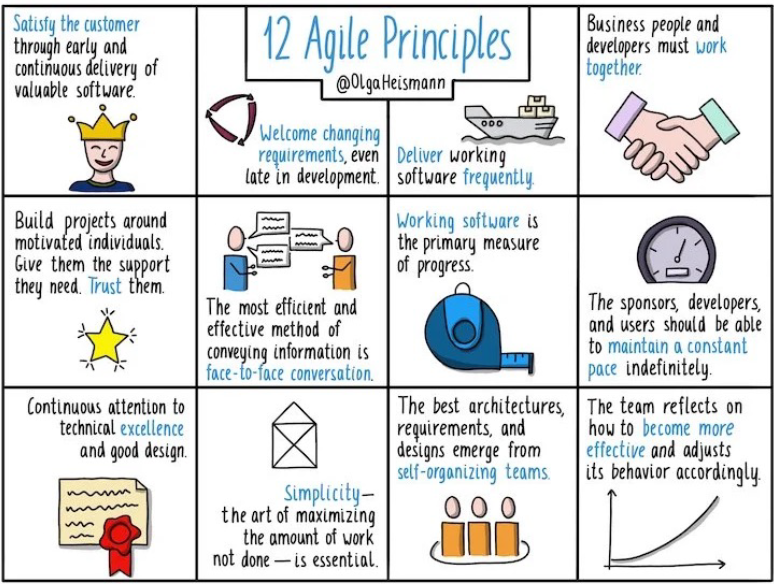
\includegraphics[scale=0.5]{20}
\end{center}

Ver analogia nos slides 6 a 15.

\pagebreak

\subsection{Técnicas de Desenvolvimento Agile}

As fases especificação, design, implementação e avaliação são intercaladas:
\begin{itemize}
  \item O sistema é desenvolvido  como uma série de versões, envolvendo
  \textbf{stakeholders} na especificaçãon e avaliação;
  \item Entregas de novas versões frequente para avaliação;
\end{itemize}

Vasto suporte de ferramentas (ex: ferramentas de testes automáticos) usado
para suportar o desenvolvimento.

\vspace{2mm}

Miníma documentação, uma vez que o foco é o código.

\begin{center}
  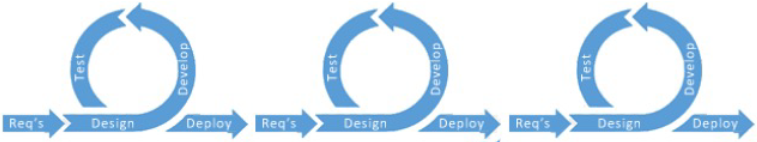
\includegraphics[scale=0.5]{21}
\end{center}

\subsubsection{Extreme Programming (XP)}

Extreme Programming (XP) é a abordagem mais utilizada para desenvolvimento
ágil de software. \textbf{Leva uma abordagem "extrema" para o desenvolvimento iterativo}:
\begin{itemize}
  \item Novas versões podem ser contruidas varias vezes por dia;
  \item Os incrementos são entregues aos clientes \uline{a cada 2 semanas};
  \item Todos os testes devem correr para cada build e cada buid apenas é aceite
  se todos os testes correrem com sucesso;
\end{itemize}

\vspace{2mm}

Utiliza uma abordagem orientada a objetos como o paradigma de desenvolvimento
preferido. Abrange um conjunto de regras e práticas que
ocorrem no contexto de quatro atividades fundamentais (framework activities):
\textbf{planning, design, coding, testing}.

\subsubsection{Release Cycle XP}

\begin{center}
  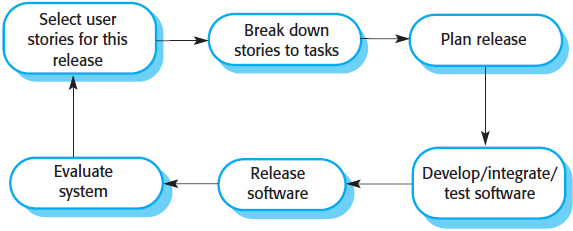
\includegraphics[scale=0.55]{22}
\end{center}

\pagebreak

\subsubsection{Práticas XP}

\begin{center}
  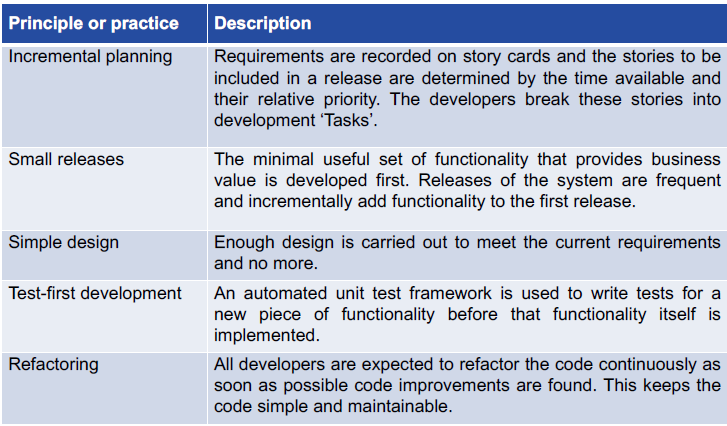
\includegraphics[scale=0.45]{23}
  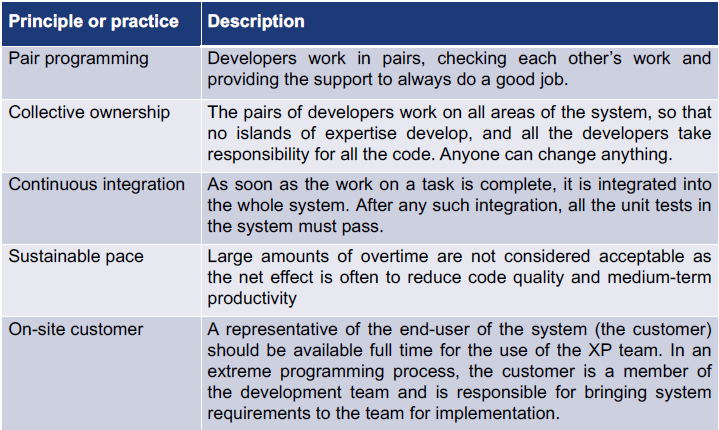
\includegraphics[scale=0.45]{24}
\end{center}

\subsubsection{Práticas influentes de XP}

Extreme Programming tem um foco técnico e não é fácil de integrar
com prática de gestão na maior parte das organizações.
Consequentemente, enquanto desenvolvimento Agile utiliza práticas
de XP, o método referido não é muito utilizado.

\vspace{2mm}

Práticas Chave:
\begin{itemize}
  \item User stories para especificação;
  \item Refatoração;
  \item Desenvolvimento Test-First;
  \item Programação em pares (pair programming);
\end{itemize}

\subsubsection{User Stories para Requisitos}

Em XP, o cliente ou user são parte da equipa XP e são
\textbf{responsáveis por tomar decisões sobre requisitos}.

\vspace{2mm}

Requisitos do user são expressos como \textbf{user stories} ou
\textbf{scenarios}. Estes são escritos em cartões e a equipa
de desenvolvimento divide-os em \textbf{tarefas de implementação}.
Estas tarefas são a base das estimativas de custo e de schedule.

\vspace{2mm}

O cliente escolhe as \textbf{stories para inclusão} na próxima release
baseado em prioridade e estimativa de schedule.

\vspace{2mm}

Exemplo slide 24 e 25.

\pagebreak

\subsubsection{Templates de User Stories}

\begin{center}
  As a \textbf{(user)}, I \textbf{(want to)}, \textbf{(so that)}.
\end{center}

\begin{itemize}
  \item \textbf{User:} Refere o user final do software;
  \item \textbf{Want to:} Refere à intenção do user, e não
  à feature que este utiliza. Temos de especificar aquilo que
  o user quer alcançar com a tarefa, sem mencionar a UI da aplicação;

  \item \textbf{So that:} Descreve a "bigger picture". Qual é o objetivo
  do user? O que é que ele quer alcançar com esta feature?
\end{itemize}


\begin{flushleft}
  \textbf{Exemplo:} As a \uline{manager}, I want to be able to
  \uline{understand my colleagues progress} so that I can
  \uline{report our success and failures}.
\end{flushleft}

\subsubsection{Organização de User Stories}

\begin{itemize}
  \item \textbf{Role-Goal-Benefit:} Força o cliente a realmente pensar
  quem é que vai beneficiar de uma feature, o que é que eles querem
  alcançar e porque é que eles querem alcançar isso;

  \item \textbf{Limites/Needs:} Subconjunto de situações que são de interesse para esta feature;
  \item \textbf{Definição de Done:} Como validar uma feature e saber que esta está concluida?
  \item \textbf{Tarefas de Engenharia:} Como esta feature interaje com outras features
  dentro do sistema ou outros subsistemas;
  \item \textbf{Estimativa de esforço:} Fornece uma medida concreta sobre o valor de uma feature;
\end{itemize}

\subsubsection{Refatoração}

Conhecimento convencional em engenharia de software é \textbf{design for change}.
Compensa gastar tempo e esforçarmo-nos a anticipar mudanças, uma vez que,
reduz o cussto mais à frente no ciclo de vida.

\vspace{2mm}

No entanto, XP mantém que este principio não compensa, uma vez que,
mudanças não podem ser previstas. Em vez disso, propõe
\textbf{melhorias contantes do código} (refactoring) para tornar
mudanças mais fáceis quando têm de ser implementadas.

\vspace{2mm}

Equipas de programação procuram por possíveis \textbf{melhorias de software}
e fazem-nas mesmo que não sejam necessárias naquele momento.
Isto melhora a \textbf{compreensão do software} e desta maneira reduz
a necessidade de documentação.

\vspace{2mm}

Mudanças são \textbf{fáceis de fazer} uma vez que o código é
\textbf{bem estruturado} e \textbf{claro}. No entanto, algumas mudanças
requerem \uline{architecture refactoring}, o que é muito mais caro.

\subsubsection*{Exemplo}

\begin{itemize}
  \item \textbf{Re-organização} de uma classe hierárquica para remover duplicação de código;
  \item \textbf{Renomear} atributos e métodos de modo a serem mais faceis de entender;
  \item \textbf{Trocar inline code} com chamadas de métodos que estão incluidas em bibliotecas;
\end{itemize}

\pagebreak

\subsubsection{Desenvolvimento Test-First}

Testar é uma parte central em XP. O \textbf{desenvolvimento test-first}:
\begin{itemize}
  \item Teste incremental é desenvolvido a partir de cenários;
  \item Envolvimento de users no desenvolvimento de testes e validação;
  \item Correr todos os testes de componente de cada vez que uma nova versão
  é built.
\end{itemize}

\begin{center}
  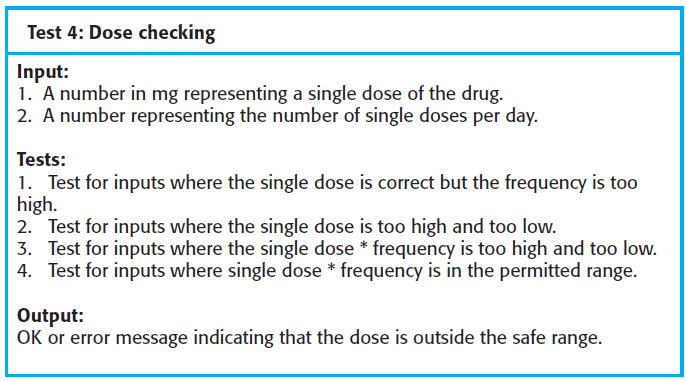
\includegraphics[scale=0.5]{25}
\end{center}

\subsubsection{Automação de Testes}

Testes são escritos como \textbf{componentes executáveis} antes da
tarefa ser implementada. Estes devem:
\begin{itemize}
  \item Ser autonomos (stand-alone);
  \item Simular a submissão de input para ser testado;
  \item Verificar que o resultado é o esperado;
\end{itemize}

Uma \textbf{automated test framework} (ex: Junit) torna mais fácil
de escrever e executar testes.

\vspace{2mm}

Uma vez que os testes são automáticos, existe um conjunto de testes
que podem ser rapidamente e facilmente executados. Quando uma nova
funcionalidade é adicionada ao sistema, todos os testes podem ser executados
e identificar problemas no novo código imediatamente.

\subsubsection{Problemas com o desenvolvimento Test-First}

\begin{itemize}
  \item Os programadores preferem programar em vez de escrever testes,
  pelo que, por vezes estes fazem \textbf{short cuts ao escrever testes}.
  Como pro exemplo, testes incompletos que não testam todas as possibilidades.

  \item Alguns testes são \textbf{muito difíceis de escrever incrementalmente}.
  Como testes para uma UI complexa, é difícil escrever testes com display logic.

  \item É dificil de julgar a \textbf{cobertura} de um conjunto de testes.
  Podemos ter muitos testes de sistema e não cobrir tudo.
\end{itemize}

\pagebreak

\subsubsection{Programação em Pares (Pair Programming)}

Um parte programadores a trabalharem juntos para desenvolver código.
Os programadores sentam se juntos num mesmo computador para desenvolver
software. Serve como uma forma de \textbf{revisão de código informal}
uma vez que cada linha de código é olhada por mais do que uma pessoa.

\vspace{2mm}

Isto ajuda a desenvolver \uline{common ownership} do código e
\uline{compreensão coletiva} pela equipa.
Reduz o risco quando um programador deixa a equipa.

\vspace{2mm}

Em pair programming, os pares são criados dinamicamente
para que todos os membros da equipa trabalhem uns com os outros durante
o processo de desenvolvimento. Encoraja a refatorização, uma vez que,
toda a equipa pode benificiar com a melhoria do código do sistema.

\vspace{2mm}

Pair programming não é necessariamente ineficiente. Estudos mostram
que um par ao trabalhar junto é mais eficiente do que dois programadores
a trabalhar separadamente.

\subsection{Gestão de Projeto Agile}

A principar responsabilidade da gestão de projeto de software é
\textbf{gerir o projeto}, para que o software \uline{seja entregue a tempo}
e dentro do \uline{budget} planeada para o projeto.

\vspace{2mm}

A abordagem tradicional para a gestão de projeto é \textbf{plan-driven}.
Define \uline{o que} deve ser entregue, \uline{quando} deve ser entregue e \uline{quem}
vai trabalhar em cada entrega.

\vspace{2mm}

A gestão de projeto Agile requer uma abordagem diferente.
É adaptada de um \textbf{desenvolvimento incremental} e as \textbf{praticas
usadas em métodos agile}.

\subsubsection{Scrum}

É um \textbf{método agile} que foca na gestão incremental do desenvolvimento.

\vspace{2mm}

Existem três fases no Scrum:
\begin{itemize}
  \item A fase inicial é o \textbf{outline planning} onde tem de se estabelecer
  os objetivos gerais para o projeto e fazer o design da arquitetura
  de software.

  \item Isto é seguido por uma serie de \textbf{ciclos sprint}, onde cada
  ciclo desenvolve um incremento do sistema.

  \item A fase de \textbf{encerramento do projeto}, termina o projeto,
  completa a documentação necessária como ajudas nos frames e manual do
  utilizador e acessa aquilo que foi aprendido com o projeto.
\end{itemize}

\begin{center}
  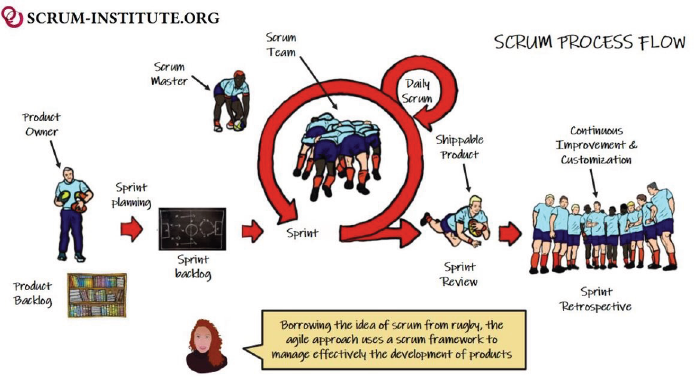
\includegraphics[scale=0.45]{26}
\end{center}

\pagebreak

\subsubsection{Scrum - Terminologia}

\begin{center}
  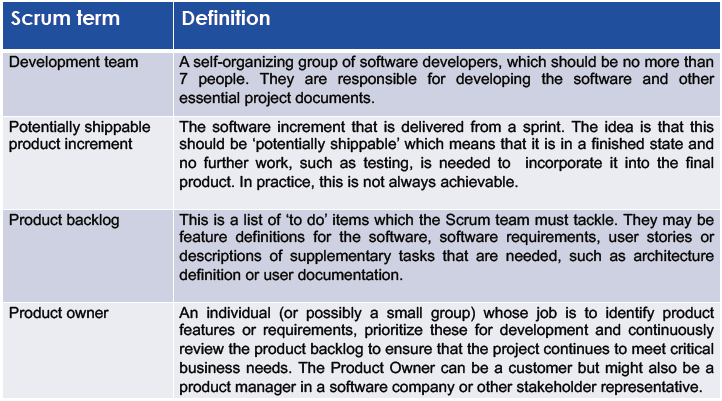
\includegraphics[scale=0.45]{27}
  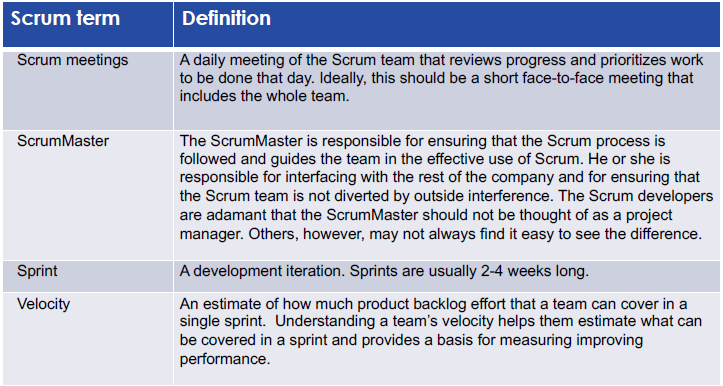
\includegraphics[scale=0.45]{28}
\end{center}

\subsubsection{Scrum sprint cycle}

\begin{center}
  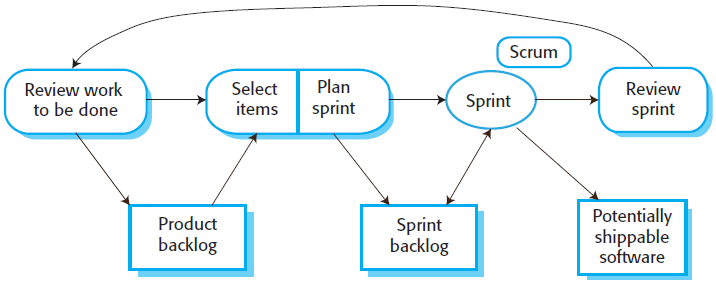
\includegraphics[scale=0.5]{29}
\end{center}

O ponto inicial ara o planeamento é o \textbf{product backlog}.
É uma lista do trabalho a ser feito no projeto.

\vspace{2mm}

A \textbf{fase selecionada} envolve toda a equipa. Quem trabalha com o
cliente para selecionar as features e as funcionalidades do
\textbf{product backlog} que vão ser desenvolvidas durante o sprint.

\vspace{2mm}

Durante a \textbf{fase de desenvolvimento}, a equipa está isolada do
cliente e da organização. Todos os canais de comunicação passam pelo
"\textbf{Scrum master}".

\vspace{2mm}

No \textbf{final do sprint}, o trabalho realizado é revisto e apresentado aos
stakeholders.

\subsubsection{Teamwork in Scrum}

O papel do \textbf{Scrum master} é proteger o a equipa de desenvolvimento
de distrações externas.
\begin{itemize}
  \item Realiza reuniões diárias;
  \item Vai verificando o backlog para ver o trabalho a ser feito;
  \item Toma decisões;
  \item Mede o progresso usando o backlog;
  \item Comunica cocm os clientes e a gestão fora da equipa;
\end{itemize}

A equipa vai a reuniões diárias curtas (\textbf{Scrums})
\begin{itemize}
  \item Membros partilham informação, descrevem o progresso/problemas
  desde a última reunião, e aquilo que estava planeado para o dia;

  \item Isto significa que todos na equipa sabem aquilo que se passa,
  os porblemas que surgiram, podem re-planear num curto tempo o trabalho;
\end{itemize}

\subsubsection{Scrum - Benefícios}

\begin{itemize}
  \item O produto é repartido num conjunto de pedaços \textbf{geriveis}. e \textbf{faceis de compreender}.
  \item \textbf{Requisitos instáveis} não prrendem o progresso;
  \item Toda a equipa tem visibilidade de tudo, consequentemente, a comunicação da equipa melhora;
  \item Os clientes vêm as entregas on-time dos incrementos, ganhando feedback em como o produto funciona;
  \item Confiança entre a equipa e o cliente, todos esperam que o projeto tenha sucesso;
\end{itemize}

\subsubsection{Kanban}

É um sistema ágil que pode ser usado para melhorar qualquer desenvolvimento
de software incluindo Scrum, XP ou Waterfall.

\vspace{2mm}

O nome "Kanban" vem do Japonês e significa "signboard" ou "billboard".
Foi usado pela primeira vez pela Toyota para Just-in-time manufacturing
plants, com o objetivo de limitar o trabalho em progresso (WIP - work in progress).

\subsubsection{Scrum vs Kanban}

Em \textbf{Scrum}, tu escolhes o trabalho que vais fazer durante o
próximo sprint antes deste começar. Depois, damos \uline{lock}
ao sprint, fazemos o trabalho todo, e passado algumas semanas
(duração normal para um sprint), a queue fica vazia.

\begin{center}
  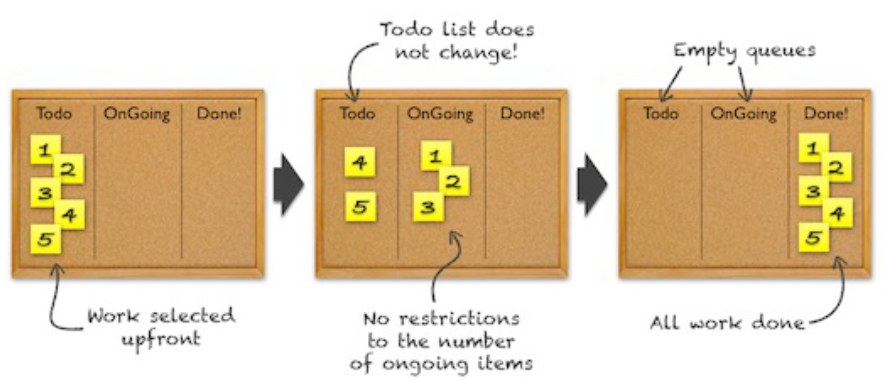
\includegraphics[scale=0.48]{30}
\end{center}

Em \textbf{Kanban}, tudo o que é limitado é o tamanho das queues,
chamado de \textbf{work in progress (WIP) limits}. Podemos alterar
os items na queue a qualquer momento, não existindo
um "fim de sprint". O trabalho continua a fluir.  

\begin{center}
  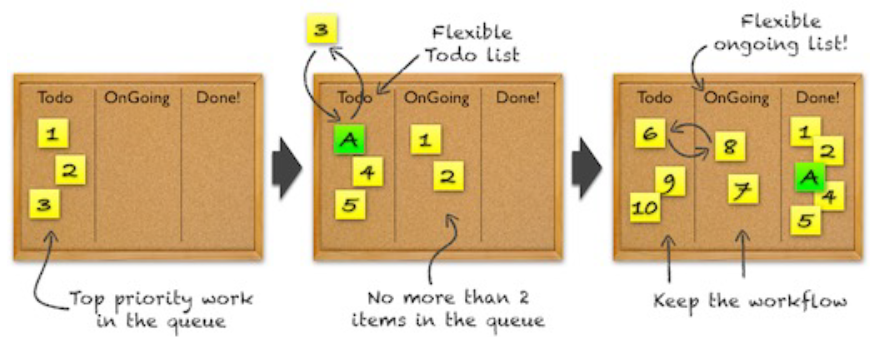
\includegraphics[scale=0.48]{31}
\end{center}


\pagebreak

\begin{center}
  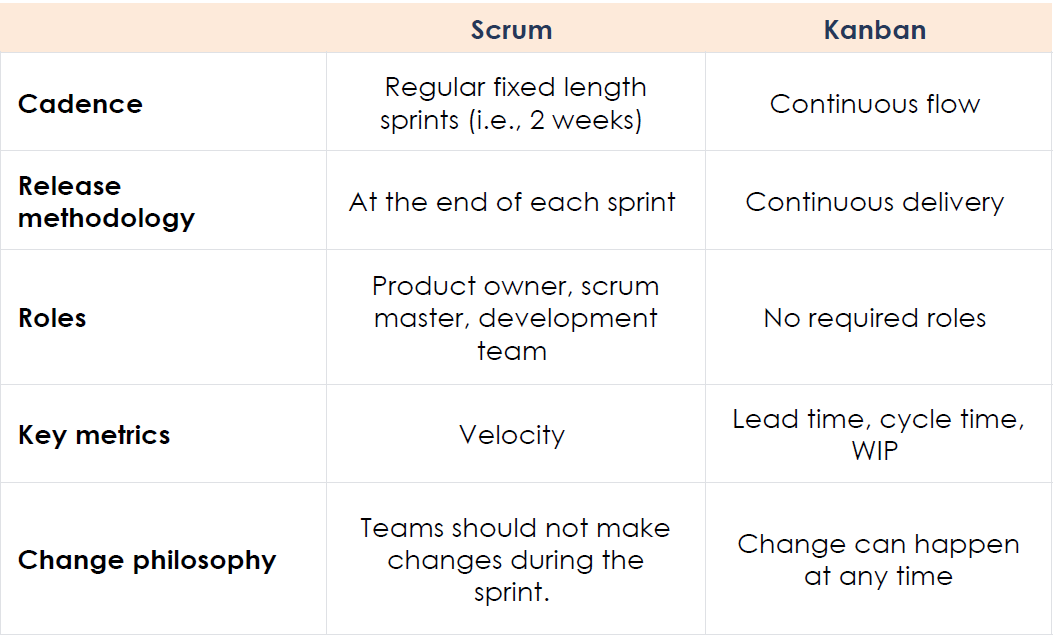
\includegraphics[scale=0.4]{32}
\end{center}

\subsection{Scaling Agile Methods}

Métodos Agile provaram ser muito eficazes para projetos
pequenos/médios, que podem ser desenvolvidos por uma equipa
pequena co-localizada.
Escalar métodos Agile involve mudar estes para poderem ser
utilizados em projetos cada vez maiores, onde existem múltiplas
equipas de desenvolvimento, podendo trabalhar até mesmo em diferentes
locais.

\vspace{2mm}

Quando escalamos métodos Agile, é importante manter fundamentos
Agile: Planeamento flexivel, releases de sistema frequentes,
integração contínua, desenvolvimento test-driven e boa comunicação
entre a equipa.

\subsubsection{Problemas de Sistema}

\begin{itemize}
  \item Quão grande é o sistema a ser desenvolvido? Métodos Agile
  \uline{são mais eficientes em equipas pequenas e co-localizadas}, em que
  ocorre uma comunicação informal.

  \item Que tipo de sistema está a ser desenvolvido? Sistemas que necessitem
  de \textbf{muita análise antes da implementação} precisam de um
  design (mais) detalhado.

  \item Qual é o tempo de vida esperado do sistema?
  \textbf{Sistemas de longa duração necessitam de documentação} para comunicar
  as intenções do sistema com os developers da equipa de suporte.

  \item O sistema está sujeito a regulamentos externos?
  Se o sistema é regulado, muito provavelmente, é necessário
  \textbf{produzir documentação detalhada} como parte do caso de segurança do
  sistema.
\end{itemize}

\subsubsection{Desenvolvimento de Sistemas Grandes}

Sistemas grandes são normalmente coleções de sistemas de comunicação separados,
onde \textbf{equipas separadas} desenvolvem cada sistema. Frequentemente,
estas equipas trabalham em locais diferentes, por vezes até em zonas com diferentes fusos horários.

\vspace{2mm}

Sistemas grandes são "\textbf{brownfield systems}" isto é,
incluem e interagem com vários sistemas existentes.
Muitos dos requisitos do sistema estão relacionados com a interação, logo
não se rendem muito à flexibilidade e desenvolvimento incremental.

\pagebreak

Sistemas grandes e os seus processos de desenvolvimento são
muitas vezes restritos por \textbf{regras e regulamentos externos},
limitando a forma como podem ser desenvolvidos.

\vspace{2mm}

Sistemas grandes tem uma \textbf{aquisição longa} e
um tempo de desenvolvimento longo também. É dificil de manter equipas
coerentes que sabem sobre o sistema durante esse periodo, uma vez que,
eventualmente, os membros vão para outros projetos ou trabalhos.

\vspace{2mm}

Sistemas grandes normalmente tem um conjunto diverso de
\textbf{stakeholders}. É praticamente impossível involver todos estes
stakeholders no processo desenvolvido.

\subsubsection{Agile: Scaling up em sistemas grandes}

\begin{itemize}
  \item Uma \uline{abordagem completamente incrementeal aos requisitos de engenharia} é \textbf{impossível};
  \item \textbf{Não pode existir} um único \uline{product owner};
  \item \textbf{Não é possível} \uline{focar apenas no código};
  \item \uline{Mecanismos de comunicação cross-team} têm de ser \textbf{designed} e \textbf{utilizados};
  \item \uline{Integração continua} é praticamente \textbf{impossível}, no entanto, é essencial
  manter builds frequentes do sistema e regular releases do sistems;
\end{itemize}

\subsubsection{Multi-team Scrum}

\begin{itemize}
  \item \textbf{Role replication}: Cada equipa tem um Product Owner para o
  seu trabalho e Scrum Master.

  \item \textbf{Product architects}: Cada equipa escolhe um arquiteto
  do produto que colaboram para desenhar e evoluir toda a arquitetura
  do sistema.

  \item \textbf{Release alignment}: As datas de releases de produtos
  de cada equipa são alinhadas de modo a demonstrar que um sistema
  completo está produzido.

  \item \textbf{Scrum of scrums}: Existe um Scrum of scrums diário, onde
  os representantes de cada equipa se encontram para discutir o progresso
  e o plano de trabalho a ser concluído.
\end{itemize}


\end{document}